\documentclass{article}
\usepackage{graphicx} % Required for inserting images
\usepackage[ruled,vlined]{algorithm2e, setspace}
\usepackage{amsthm, amssymb, amsmath}

\begin{document}

\section{Extra files}

\begin{figure}[htbp]
    \centering
    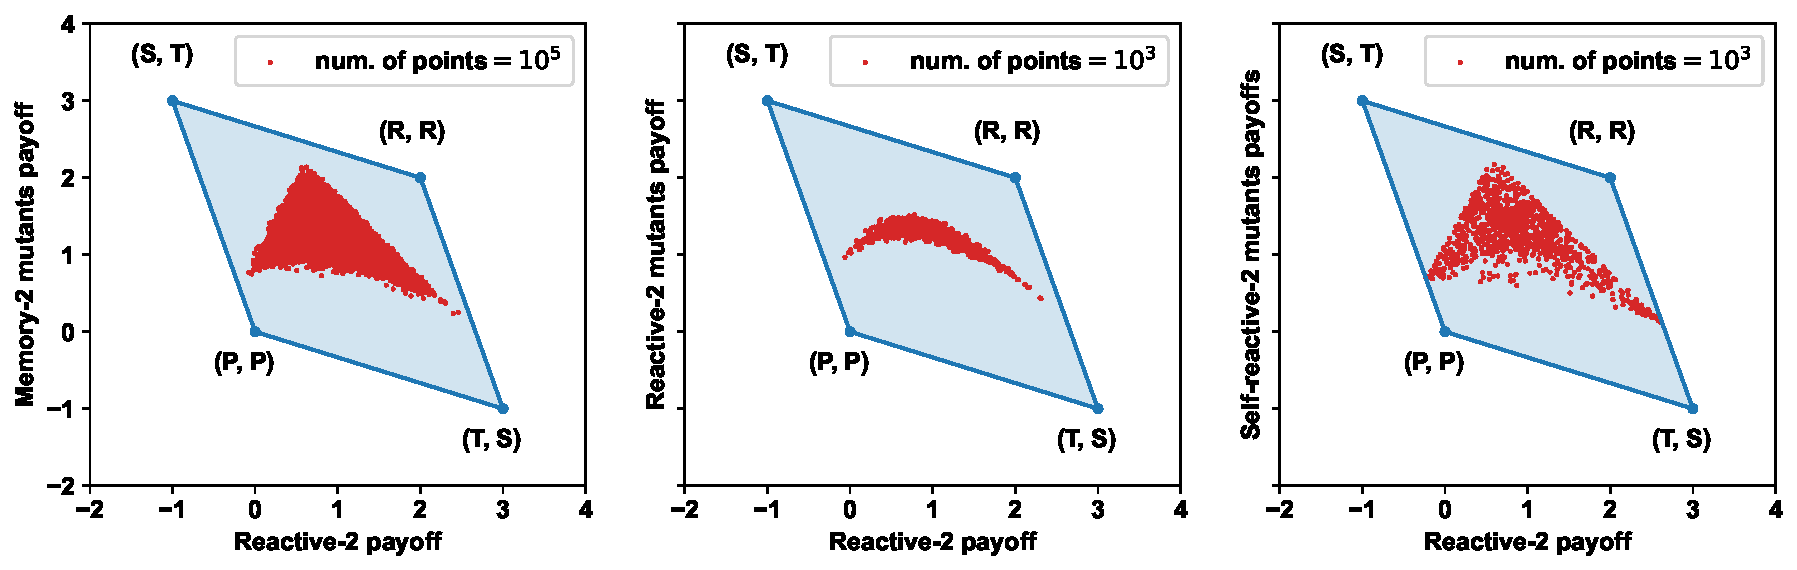
\includegraphics[width=\textwidth]{figures/sufficiency_of_self_reactive_numerical_example_n_2.pdf}
    \caption{Parameters: $b=3, c=1$ and $\mathbf{p}=(0.37, 0.89, 0.95, 0.23)$}
    \label{fig:enter-label}
\end{figure}


\begin{algorithm}[H]
    \setstretch{1.35}
      \SetKwInOut{Input}{input}
      \Input{$\mathbf{p}, n$}
      pure\_self\_reactive\_strategies $\gets \left\{ \mathbf{\tilde{p}} ~\big|~ \mathbf{\tilde{p}} \in \{0, 1\}^{2 ^ n} \right\}$ \;
      isNash $\gets$ True \; 
      \For{$\mathbf{\tilde{p}} \in$ pure\_self\_reactive\_strategies}{
      \uIf{$ \pi(\mathbf{p}, \mathbf{p}) \leq \pi(\mathbf{\tilde{p}}, \mathbf{p})$}{
        condition $\gets$ False \;
      }
      \Else{
        condition $\gets$ True \;
      }
      isNash $\gets$ isNash AND condition\;
      }
      \Return (\(\mathbf{p}\), isNash) \;
      \caption{Nash Evaluation for a reactive$-n$ strategy.}
    \end{algorithm}

\end{document}
